
\section{Usabilità su mobile}
	Poiché oggi la maggioranza dell'utenza naviga con dispositivi mobili questa sezione è d'obbligo. 
	In ambito mobile i problemi di usabilità prima affrontati si amplificano, per motivi di sintesi quindi si è analizzato la \textbf{mobile responsiveness} e i \textbf{tempi di caricamento}, caratteristiche che ritengo essenziali per l'usabilità in ambiente mobile.

	\subsection{Responsiveness}
		Il layout del sito degrada elegantemente e si nota lo sforzo attuato per garantire una gradevole navigazione su mobile senza sacrificare il layout. Sottoporre la homepage al test dello strumento online di Google \href{https://www.google.com/webmasters/tools/mobile-friendly/?hl=it}{Mobile Friendly} fa guadagnare il massimo punteggio, ogni accortezza proposta da Google è implementata.
		
	\subsection{Tempi di caricamento}
		Molto male invece nei tempi di caricamento, lo strumento \href{https://developers.google.com/speed/pagespeed/insights/}{SpeedTest} assegna un punteggio di 37 punti su 100. 
		
		I tempi di caricamento della sola homepage usufruendo di una connessione wi-fi con uno smartphone di fascia bassa misurano più di 10 secondi, ulteriori test con telefoni più prestanti e sempre con connessione wi-fi misurano quasi 10 secondi. Un'enormità se consideriamo che l'utente medio concede solo 2 secondi di attesa.
		
		La causa di questo possiamo individuarla nella dimensione della pagina:
		La homepage pesa più di 3 MB come mostra la figura (figura \ref{fig:PerformanceEmptyCache}) e il caching non garantisce un risparmio significativo (figura \ref{fig:PerformanceWithCache}). Il sito in generale contiene troppo codice Javascript e troppe immagini non compresse e nella maggior parte dei casi di troppo. Alcuni possibili rimedi immediati sono:
		\begin{itemize}
			\item delegare il download delle librerie Javascript a server più prestanti in modo da alleggerire le trasmissioni dal sito e velocizzare i tempi di download;
			\item comprimere le immagini o meglio ridurne la presenza in tutte le pagine del sito;
			\item comprimere tutti i file scaricati alla visita di una pagina (CSS, JAvascript ecc.), sfruttando strumenti che eliminano gli spazi inutili per esempio;
			\item raggruppare tutti i file scaricati alla visita di una pagina in un unico file così da evitare continue richieste client-server.
		\end{itemize}
		
		\begin{figure}
			\centering
			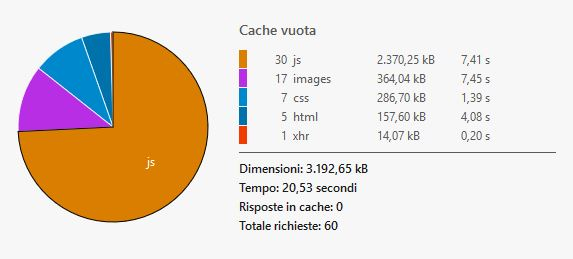
\includegraphics[scale=0.8]{images/PerformanceEmptyCache}
			\caption{Dimensione file di download per la homepage}
			\label{fig:PerformanceEmptyCache}
		\end{figure}		
		
		\begin{figure}
			\centering
			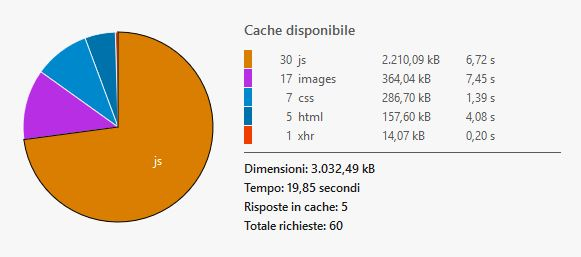
\includegraphics[scale=0.8]{images/PerformanceWithCache}
			\caption{Dimensione file di download per la homepage con l'uso della cache}
			\label{fig:PerformanceWithCache}
		\end{figure}